
\documentclass[8pt,a4paper]{article}
\usepackage{fullpage}
\usepackage{indentfirst} %首段縮排
\usepackage[top=1.5cm, bottom=1.5cm, left=1.5cm, right=1.5cm]{geometry}
\usepackage{amsmath,amsthm,amsfonts,amssymb,amscd,longtable}
\usepackage{lastpage}
\usepackage{enumerate}
\usepackage{fancyhdr}
\usepackage{mathrsfs}
\usepackage{mathtools}
\usepackage{multicol}
\usepackage{xcolor}
\usepackage{bookmark}
\usepackage{verbatim}
\usepackage{float}  % in order to use H for figure position
\usepackage{graphicx}
\DeclareGraphicsExtensions{.pdf,.jpg,.png,.mps} % Portable Document Format,
%\usepackage{luacode}  % This can not let Reference to be showed by Butters
\usepackage{multirow}
\usepackage{makecell}
\usepackage{listings}
\usepackage{multicol}
\usepackage{hyperref}
\usepackage{caption}
\usepackage{xeCJK} %For Traditional Chinese in XeLaTeX
\setCJKmainfont{MingLiU} %For Traditional Chinese in XeLaTeX
\setCJKsansfont{Microsoft JhengHei} %For Traditional Chinese in XeLaTeX

% BibTeX
%\usepackage{bibentry} %Function unknown added by Per Sahlholm
%\usepackage[round,authoryear]{natbib} %Nice author (year) citations
\usepackage[square,numbers]{natbib} %Nice numbered citations
%\usepackage{cite} % Make references as [1-4], not [1,2,3,4]
%\newcommand{\bibspace}{\vspace{2mm}}
\bibliographystyle{unsrtnat} % Unsorted bibliography by Butters
%\bibliographystyle{plainnat} %Choose for including URLs   %Commented by Butters
%\bibliographystyle{unsrt} 
%\bibpunct{[}{]}{,}{y}{,}{,}
%\renewcommand{\bibsection}{} %Removes the References chapter title
%\usepackage[numbib,notlof,notlot,nottoc]{tocbibind} %Adds number to bibliography

\let\ds\displaystyle
\usepackage[shortlabels]{enumitem}
% \pagenumbering{gobble} % Remove page number

\pagestyle{plain}
\hypersetup{
  colorlinks=true,
  linkcolor=blue, 
  citecolor=blue,% new
  linkbordercolor={0 0 1}
}

\begin{document}

\title{ \bf{ Feedforward Control Final Project \\  Decoding Hand movement with Wiener Filter }}
\author{ Hsi-Chih Wu 伍錫志 \\ Department of Mechanical Engineering, National Cheng Kung University \\ Email: N16074988@gs.ncku.edu.tw  }
\date{}

\maketitle

\section*{Abstract}
\bookmark[level=chapter,page=\arabic{page}]{Abstract}

This reseach used Wiener filter to decode the hand movement of the monkey, with invasive electrode implanted in its brain. 
With the help of iterative control, the weights of the Wiener filter can be adjusted, and the error approach to minimum.

\begin{multicols}{2}

\section*{Introduction}
\bookmark[level=chapter,page=\arabic{page}]{Introduction}

Brain machine interface (BMI) 

\section*{Dataset}
\bookmark[level=chapter,page=\arabic{page}]{Dataset}

We use the open source dataset, \href{https://zenodo.org/record/583331#.XWirEigzZPb}{Nonhuman Primate Reaching with Multichannel Sensorimotor Cortex Electrophysiology}, 
publised by the author of \cite{makin2018}. Two monkeys, Indy and Loco, performed hand-reaching tasks for several minutes. 
The neural data was recorded using 96-channel silicon microelectrode array, and the self-reaching was performed in a  $8 \times 8$ virtual grid, illustrated in Figure \ref{fig:monkey_drawing}.
The panel was placed between the monkeys' hand and their eyes, making the monkeys unable to actual see its arms during the experiment period. 
The neurla signal was sampled at 24.4kHz and the fingertip position was sampled at 250Hz. 
An IIR bandpass filter was then used to extract signal from 500Hz to 5000Hz from the raw neural signal, and determined a threhold value, to isolate spike units. 
37 sessions of monkey Indy's spike train data and 10 sessions of monkey Loco's are provided from the website.  
However, only 30 sessions of monkey Indy still have its raw neural signal remain, while the rest raw data are unfortunately lost. 
This reseach only consider the sorted spike train session as input, refrain from doing other signal processing techniques on our own.


\begin{figure}[H]
  \begin{center}
      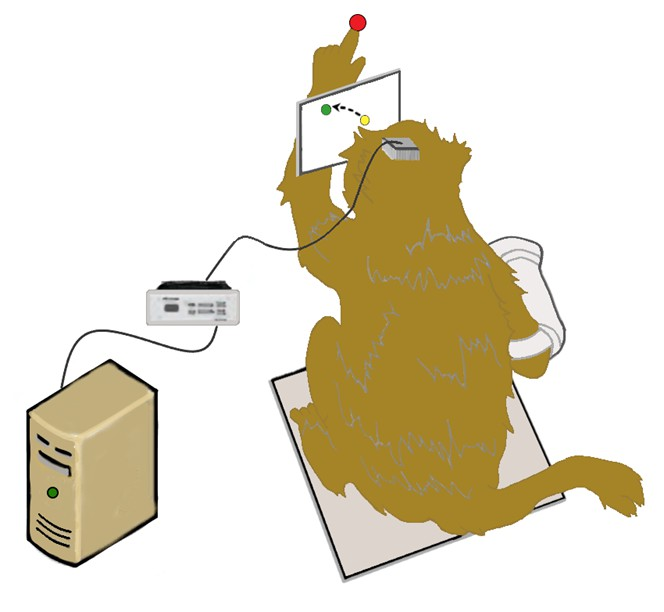
\includegraphics[width=150pt]{./Figures/monkey.jpg}
      \caption{Animal Experiment}
      \label{fig:monkey_drawing}
  \end{center}
\end{figure}


\section*{Method}
\bookmark[level=chapter,page=\arabic{page}]{Method}

The Wiener filters are linear least square filters which can be used for prediction, estimation, interpolation, signal and noise filtering and so forth.\cite{widrow1987}
The impulse response of a FIR filter can be expressed algebraically as 

\begin{align}
  \begin{split}
  g_{k} &= f_{k}h_{0} + f_{k-1}h_{1} + f_{k-2}h_{2} + \cdots \\
        &= \sum_{l=0}^{\infty} f_{k-l}h_{l}
  \end{split}
\end{align}
Which is a convolution of the input signal $f_{k}$ with the impulse response $h_{k}$, can be represented as

\begin{align}
\label{eq:conv}
  g_{k} &= f_{k} * h_{k} 
        = \sum_{l=0}^{\infty} f_{k-l}h_{l} 
\end{align}

The z-transform of the input $f_{k}$ is defined as

\begin{align}
  \label{eq:z-transform}
  F(z)&\triangleq \sum_{k=-\infty}^{\infty} f_{k}z^{-k}
\end{align}

The z-transform of the output signal $g_{k}$ can be obtained from convolution in equation \ref{eq:conv} and in equation \ref{eq:z-transform}. Thus, 

\begin{align}
  \begin{split}
  G(z)&\triangleq \sum_{k=-\infty}^{\infty} g_{k}z^{-k}\\
      &=\sum_{k=-\infty}^{\infty} z^{-k} \sum_{l=0}^{\infty} f_{k-l}h_{l} \\
      &=\sum_{k=-\infty}^{\infty} \sum_{l=0}^{\infty} z^{-k}f_{k-l}h_{l}
  \end{split}
\end{align}

After z-transform, the above can be express as

\begin{align}
  G(z) &= H(z) \cdot F(z)
\end{align}

Now we will deprive the autocorrelation of input signal, crosscorrelation between input and output signal, and autocorrelation of output. 

\subsection*{input autocorrelation}
\bookmark[level=1,page=\arabic{page}]{input autocorrelation}
First, we define the autocorrelation of $f_{k}$ as

\begin{align}
  \phi_{ff}(m) &\triangleq E \left[ f_{k} \cdot f_{k+m} \right]
\end{align}

where the symbo $E[\cdot]$ represents expectation. The autocorrelation function can also be expressed as time average:

\begin{align}
  \phi_{ff}(m) &= \lim_{N\rightarrow\infty} \frac{1}{2N+1} \sum_{l=-N}^{N} f_{k-l} \cdot f_{k-l+m}
\end{align}

\subsection*{input-output crosscorrelation}
\bookmark[level=1,page=\arabic{page}]{input-output crosscorrelation}

Second, the crosscorrelation function between input $f_{k}$ and the output $g_{k}$ is defined as


\begin{align}
  \phi_{fg}(m) &\triangleq E \left[ f_{k} \cdot g_{k+m} \right] = \phi_{gf}(-m)
\end{align}

Using equation \ref{eq:conv}, this can be express as

\begin{align}
  \begin{split}
    \phi_{fg}(m) &= E \left[ f_{k} \sum_{t=0}^{\infty} f_{k-l+m}h_{l} \right]\\
    &= E \left[ \sum_{l=0}^{\infty} h_{l} f_{k} f_{k-l+m} \right]
  \end{split}
\end{align}

and since $h_{t}$ is fixed for all $ l $, and since $f_{k}$ is stohastic, the expression can be writted as

\begin{align}
  \label{eq:input_output_crosscorrelation}
  \begin{split}
    \phi_{fg}(m) &= \sum_{l=0}^{\infty} h_{l} E \left[ f_{k} f_{k-l+m} \right] \\
    &= \sum_{l=0}^{\infty} h_{l} \phi_{ff}(m-l) \\
    &= h_{m} * \phi_{ff}(m)
  \end{split}
\end{align}

The crosscorrelation between input and output of a linear digitial filter is the convolution of the input autocorrelation function with the impulse response.
Taking the z-transform of equation \ref{eq:input_output_crosscorrelation}, we can get 

\begin{align}
  \Phi_{fg}(z)&=H(z) \cdot \Phi_{ff}(z)
\end{align}

\subsection*{output autocorrelation}
\bookmark[level=1,page=\arabic{page}]{output autocorrelation}
Third, the autocorrelation function of the output of the digitial filter is

\begin{align}
  \label{eq:output_autocorrelation}
  \begin{split}
    \phi_{gg}(m)&= E \left[ g_{k} \cdot g_{k+m} \right] \\
                &= E \left[  \sum_{l=0}^{\infty} f_{k-l}h_{l} \sum_{\mu=0}^{\infty} f_{k-\mu+m}h_{\mu}  \right] \\
                &= \sum_{l=0}^{\infty} \sum_{\mu=0}^{\infty} h_{l} h_{\mu} E \left[ f_{k-l} f_{k-\mu +m} \right] \\
                &= \sum_{l=0}^{\infty} \sum_{\mu=0}^{\infty} h_{l} h_{\mu} \phi_{ff}(m+l-\mu) \\
                &= \sum_{l=0}^{\infty} h_{l} \sum_{\mu=0}^{\infty} h_{\mu} \phi_{ff}(m+l-\mu)
  \end{split}
\end{align}

Combining equation \ref{eq:input_output_crosscorrelation} and equation \ref{eq:output_autocorrelation}, we obtained

\begin{align}
  \label{eq:output_autocorrelation_2}
  \phi_{gg}(m) &= \sum_{l=0}^{\infty} h_{l} \phi_{fg}(m+l)
\end{align}

equation \ref{eq:output_autocorrelation} is similar to a convolution. In order to auctually make it a convolution form, we define a time-reversed impuse response as

\begin{align}
  \begin{split}
  \tilde{h}_{l} &\triangleq h_{-l}, or \\
  \tilde{h}_{-l} &\triangleq h_{l}
  \end{split}
\end{align}

so accordingly, 

\begin{align}
  \label{eq:output_conv}
  \begin{split}
    \phi_{gg}(m) &= \sum_{l=0}^{\infty} \tilde{h}_{-l} \phi_{fg}(m+l) \\
    &= \sum_{l=0}^{-\infty} \tilde{h}_{l} \phi_{fg}(m-l)
  \end{split}
\end{align}

Since equation \ref{eq:output_conv} is a convolution, it can be written as

\begin{align}
  \label{eq:tilde_output_conv}
  \begin{split}
    \phi_{gg}(m) &= \tilde{h}_{l} * \phi_{fg}(m) \\
    &= h_{-m} * \phi_{fg}(m)
  \end{split}
\end{align}


Combining equation \ref{eq:input_output_crosscorrelation} and equation \ref{eq:tilde_output_conv}, it becomes 

\begin{align}
  \label{eq:double_conv}
  \phi_{gg}(m) &= h_{-m} * h_{m} * \phi_{ff}(m)
\end{align}

which is a double convolution.

Implementing z-transform to equation \ref{eq:double_conv}, it becomes

\begin{align}
  \Phi_{gg}(z) &= H(z^{-1}) \cdot H(z) \cdot \Phi_{ff}(z)
\end{align}


\subsection*{Two-sided Wiener Filters}
\bookmark[level=1,page=\arabic{page}]{Two-sided Wiener Filters}

The error is defined as the difference between filter output and the desired response, showed in Fig \ref{fig:wiener}

\begin{align}
  \label{eq:error}
  \epsilon_{k} &= d_{k} - g_{k}
\end{align}


\begin{figure}[H]
  \begin{center}
      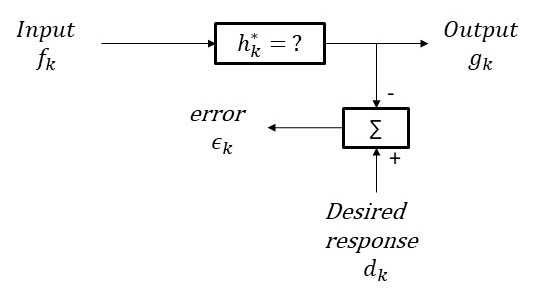
\includegraphics[width=200pt]{./Figures/wiener.jpg}
      \caption{}
      \label{fig:wiener}
  \end{center}
\end{figure}


and the impulse response of the Wiener filter is obtained by finding an expresssion for mean square error and minimizing this wirth repect to the impulse response. 
Squaring both sides of equation \ref{eq:error} and using equation \ref{eq:conv}, we get

\begin{align}
  \begin{split}
    \epsilon_{k}^{2}&= d_{k}^{2} + g_{k}^{2} -2d_{k}g_{k} \\
    &= d_{k}^{2} + \sum_{l=-\infty}^{\infty} \sum_{\mu=-\infty}^{\infty} h_{l}h_{\mu}f_{k-l}f_{k-\mu} \\ 
    &\quad -2 \sum_{l=-\infty}^{\infty} h_{l}f_{k-l}d_{k}
  \end{split}
\end{align}

Taking expectation of both sides yields an expression for mean square error (MSE):

\begin{align}
  \begin{split}
      E \left[ \epsilon_{k}^{2} \right] &= E \left[ d_{k}^{2} \right] + \sum_{l=-\infty}^{\infty} \sum_{\mu=-\infty}^{\infty} h_{l} h_{\mu}  E \left[ f_{k-l} f_{k-\mu} \right] \\ 
      &\quad  -2 \sum_{l=-\infty}^{\infty} h_{l} E \left[ f_{k-l} d_{k}  \right] \\
      &= \phi_{dd}(0) + \sum_{l=-\infty}^{\infty} \sum_{\mu=-\infty}^{\infty} h_{l}h_{\mu} \phi_{ff}(l-\mu) \\
      &\quad  -2 \sum_{l=-\infty}^{\infty} h_{l}\phi_{fd}(l)
  \end{split}
\end{align}

The partial derivative of the MSE with respect to the $j$th impulse of the filter impulse response, 

\begin{align}
  \begin{split}
  \frac{ \partial E \left[ \epsilon_{k}^{2} \right]  }{ \partial h_{j} } &= 0 + 2 \sum_{l=-\infty}^{\infty} h_{l} \phi_{ff}(j-1) \\
  &\quad -2 \phi_{fd}(j)
  \end{split}
\end{align}

We must set this derivative to zero for all values of $j$. The result is the Wiener impulse response $h_{k}^{*}$, determined by

\begin{align}
  \sum_{l=-\infty}^{\infty} h_{l}^{*} \phi_{ff}(j-l) &= \phi_{fd}(j),\ for\ all\ j
\end{align}

This is the Wiener-Hopf equation, and it is in the convolution Format

\begin{align}
  h_{k}^{*} * \phi_{ff}(k) &= \phi_{fd}(k)
\end{align}

after takin z-transform of both sides

\begin{align}
  \begin{split}
    H^{*}(z) \cdot \Phi_{ff}(z) &= \Phi_{fd}(z),\ or \\
    H^{*}(z) &= \frac{ \Phi_{fd}(z) }{ \Phi_{ff}(z)  }
  \end{split}
\end{align}

and $H^{*}(z)$ is the transfer function of the Wiener filter, which is easily obtained from the z-transforms of the autocorrelation function of the input signal and the crosscorrelation function of between the input and desired response. 
The Wiener impulse response can be obtained by inverse z-transform of $H^{*}(z)$.

\subsection*{Linear Modeling for BMI and the Wiener Filter}
\bookmark[level=1,page=\arabic{page}]{Linear Modeling for BMI and the Wiener Filter}


\section*{Results}
\bookmark[level=chapter,page=\arabic{page}]{Results}


\section*{Conclustion}
\bookmark[level=chapter,page=\arabic{page}]{Conclustion}

\bibliography{./reference} \label{sec:references}
\bookmark[level=chapter,page=\arabic{page}]{References}
\newpage


\end{multicols}

\end{document}